% 在工作中经常会遇到pdf文档提取页面,拆分,以及合并。但是网上很多的工具都是收费的,在这里为大家提供一种pdf提取与合并的实用工具. 有很多的博客或帖子介绍了如何处理pdf文件, 但是这些工作只是部分介绍了一种(或合并或提取工作),本人加入自己的理解并完善。注:这里的代码均可在latex与cTex环境运行.

\documentclass[a4paper]{article}% or something else
\usepackage{pdfpages}    % need this package
\begin{document}

% 提取pdf文档
%  所有页
%\includepdf[pages=-]{test1.pdf}
% 单页 第一页
%\includepdf[pages={1}]{test1.pdf}
% 单页 第5页
%\includepdf[pages={5}]{test1.pdf}
%  1,2,4页
%\includepdf[pages={1,2,4}]{test1.pdf}
%  1到3页
%\includepdf[pages={1-3}]{test1.pdf}
%  多种方法结合, {}代表空页面
%\includepdf[pages={3,{},8-11,15}]{test1.pdf}

%合并pdf文档
% 完整合并
%\includepdf[pages=-]{test1.pdf}
%
\includepdf[pages=-]{test2.pdf}
% 这里合并提取是在同一个文件夹下完成的。当然,我们也可以对要操作的pdf文件加上路径
% \includepdf[pages={1,2}]{file2pdf/test1.pdf}
% 
\includepdf[pages={3,4}]{file2pdf/test2.pdf}

% 部分合并,合并test1文档1,2页和test2文档3,4页
\includepdf[pages={1,2}]{test1.pdf}

\includepdf[pages={3,4}]{test2.pdf}
\end{document}
